\section*{Task 3a} % (fold)
\label{sec:Task 3a}
	
	\begin{figure}[h]
		\begin{center}
			\newlength\figureheight 
			\newlength\figurewidth 
			\setlength\figureheight{6cm} 
			\setlength\figurewidth{9cm} 
			% This file was created by matlab2tikz v0.2.0.
% Copyright (c) 2008--2012, Nico Schlömer <nico.schloemer@gmail.com>
% All rights reserved.
% 
% 
% 
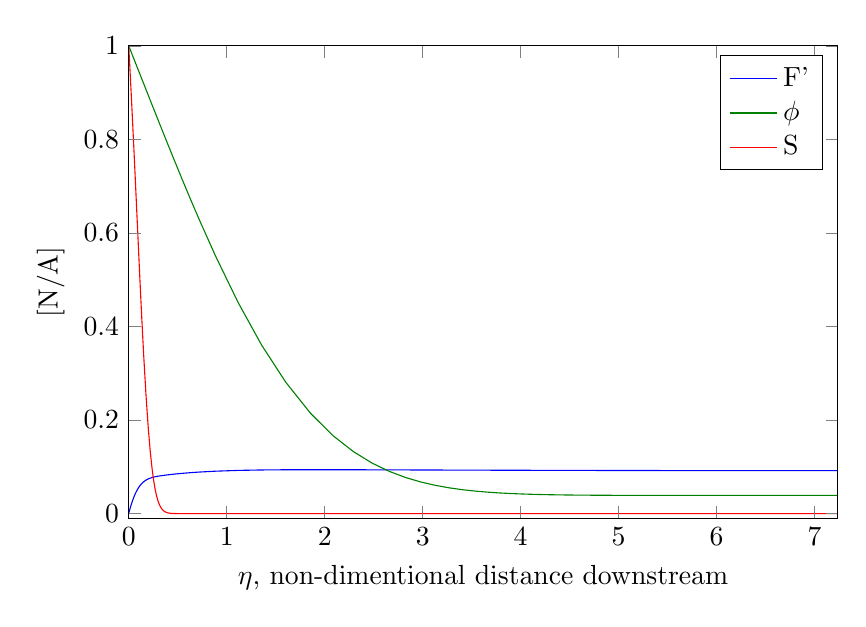
\begin{tikzpicture}

\begin{axis}[%
width=\figurewidth,
height=\figureheight,
scale only axis,
xmin=0, xmax=7.232268737012,
xlabel={$\eta$, non-dimentional distance downstream},
ymin=-0.01, ymax=1,
ylabel={[N/A]},
axis on top,
legend style={nodes=right}]
\addplot [
color=blue,
solid
]
coordinates{
 (0,0)(0.00142151536207323,0.00116653416956551)(0.00852909217243939,0.00681001089873038)(0.02366227352376,0.0178095218684272)(0.0410432016771387,0.0288291429148925)(0.0584280465823158,0.0382583750517365)(0.0751944429660008,0.0459790538649775)(0.0870253046482391,0.0506876282710513)(0.0988561663304774,0.0548402811785791)(0.112159699456503,0.058905579699678)(0.12983893801221,0.0634304941045272)(0.152276694934361,0.0679496308998799)(0.177475992166274,0.071720722020685)(0.200299571052782,0.0742301401777152)(0.220666457260637,0.0759345600970439)(0.238873300370454,0.0771440754324363)(0.25530899284643,0.0780470265413464)(0.27032139418118,0.0787541833252786)(0.284184165031273,0.0793312832657877)(0.297104462004813,0.0798184554341587)(0.309238905372862,0.0802410460034099)(0.320707465374234,0.0806156165295333)(0.331603653331698,0.0809533376906284)(0.342001661835006,0.0812619677633093)(0.351961341043679,0.0815470425161679)(0.361531702386247,0.0818126121574614)(0.37075342451793,0.0820617101217081)(0.379660676772656,0.0822966585553783)(0.388282468885137,0.0825192717846755)(0.396643666254217,0.0827309945609372)(0.40476576518225,0.0829329977337645)(0.412667493087218,0.0831262456072185)(0.420365279193378,0.083311544134307)(0.42787362791949,0.0834895759343099)(0.435205418282192,0.0836609261141848)(0.442372146367658,0.0838261015820298)(0.449384123453311,0.0839855456919073)(0.456250639264069,0.0841396494973528)(0.462980097551305,0.0842887605107307)(0.469580129460632,0.0844331896052112)(0.476057689005694,0.0845732165190222)(0.482419133922059,0.0847090942939108)(0.488670294590823,0.0848410528939596)(0.4948165330539,0.0849693021849899)(0.501118122371576,0.0850992707813553)(0.507875887788803,0.0852369530045107)(0.515170951373743,0.0853836342388603)(0.52311047227652,0.0855410010792832)(0.531837208658068,0.0857112712909797)(0.541547139880878,0.0858974449651891)(0.552519355517513,0.0861037227540903)(0.565169973299464,0.0863362442999506)(0.58015718392977,0.0866044896586391)(0.598607434641521,0.0869241983214461)(0.622673331920724,0.0873242563845964)(0.657209724195049,0.0878660916583559)(0.716723208841552,0.0887157864412036)(0.885511414941763,0.0906255558742339)(1.11559704696663,0.0922917647579597)(1.35657880378265,0.0932363639259047)(1.60324268556716,0.0936745855932849)(1.85567525515445,0.0938023852711316)(2.08434217916761,0.093764558385681)(2.29169549068954,0.0936649089802003)(2.4820284756292,0.0935462588177733)(2.65870784546609,0.0934256486603753)(2.82420902482359,0.0933096874543431)(2.98037103466579,0.0932006720211203)(3.12859153543315,0.0930991008554218)(3.26995750253231,0.0930047418904259)(3.40533202831783,0.092917094887158)(3.53541300941441,0.0928355913548978)(3.66077376479881,0.0927596780576579)(3.78189181414427,0.092688848455865)(3.89916971934952,0.0926226511105586)(4.01295048207048,0.0925606883144474)(4.12352912547211,0.0925026110117608)(4.23116154835446,0.092448112727482)(4.33607139300889,0.0923969236683217)(4.43845544343723,0.0923488054335547)(4.53848791901935,0.0923035464407221)(4.6363239269866,0.0922609580746184)(4.73680153586433,0.0922189455615148)(4.8440950753594,0.0921760135130969)(4.95945231695988,0.0921320786559433)(5.08450939456351,0.0920870522585633)(5.22144996299879,0.0920408527988155)(5.37327889001518,0.0919934251361811)(5.54428895347899,0.0919447837211118)(5.74090804795748,0.0918951134793378)(5.97336331782887,0.0918450214085049)(6.25930422222351,0.0917962306874594)(6.63288076019851,0.0917538066037377)(7.17268776448588,0.0917351701756223)(7.232268737012,0.0917362034568848) 
};

\addlegendentry{F'};

\addplot [
color=green!50!black,
solid
]
coordinates{
 (0,1)(0.00142151536207323,0.999247295315158)(0.00852909217243939,0.995483531382042)(0.02366227352376,0.987468568268171)(0.0410432016771387,0.978261126972536)(0.0584280465823158,0.96904984989953)(0.0751944429660008,0.960165121368419)(0.0870253046482391,0.953895467755127)(0.0988561663304774,0.947625844990646)(0.112159699456503,0.940576195574473)(0.12983893801221,0.931209225092491)(0.152276694934361,0.919324986004269)(0.177475992166274,0.905986140682609)(0.200299571052782,0.893915082615721)(0.220666457260637,0.883153928605581)(0.238873300370454,0.873544278890128)(0.25530899284643,0.864879026255018)(0.27032139418118,0.856973085116734)(0.284184165031273,0.849680899872117)(0.297104462004813,0.842892293886193)(0.309238905372862,0.836523959626854)(0.320707465374234,0.830512071195124)(0.331603653331698,0.824806866366973)(0.342001661835006,0.819368851774819)(0.351961341043679,0.814166158476917)(0.361531702386247,0.80917268014212)(0.37075342451793,0.804366741393812)(0.379660676772656,0.799730128780576)(0.388282468885137,0.795247373442648)(0.396643666254217,0.790905211479829)(0.40476576518225,0.786692171851313)(0.412667493087218,0.782598257277699)(0.420365279193378,0.778614693970611)(0.42787362791949,0.774733733071915)(0.435205418282192,0.770948491414434)(0.442372146367658,0.767252822543876)(0.449384123453311,0.763641211316149)(0.456250639264069,0.760108687030483)(0.462980097551305,0.756650751278571)(0.469580129460632,0.753263317604064)(0.476057689005694,0.749942660678772)(0.482419133922059,0.746685373254216)(0.488670294590823,0.743488329459935)(0.4948165330539,0.740348653372356)(0.501118122371576,0.737133497152385)(0.507875887788803,0.733690026946056)(0.515170951373743,0.729978008766879)(0.52311047227652,0.725944353366645)(0.531837208658068,0.721518460056169)(0.541547139880878,0.716603603115512)(0.552519355517513,0.711062360003955)(0.565169973299464,0.704690404947095)(0.58015718392977,0.697165643970387)(0.598607434641521,0.687939216325888)(0.622673331920724,0.675968382442628)(0.657209724195049,0.658921760513496)(0.716723208841552,0.629939170671103)(0.885511414941763,0.550835471784033)(1.11559704696663,0.451648768917668)(1.35657880378265,0.360131744451815)(1.60324268556716,0.280671293883516)(1.85567525515445,0.214355566654556)(2.08434217916761,0.166683344123815)(2.29169549068954,0.132640900855074)(2.4820284756292,0.108113102038916)(2.65870784546609,0.0902734765329914)(2.82420902482359,0.0771950646724941)(2.98037103466579,0.0675449934053189)(3.12859153543315,0.0603868302992522)(3.26995750253231,0.055053822992063)(3.40533202831783,0.0510660088705673)(3.53541300941441,0.0480747868767)(3.66077376479881,0.0458251018664368)(3.78189181414427,0.0441292040297042)(3.89916971934952,0.0428481821282067)(4.01295048207048,0.0418788149818723)(4.12352912547211,0.0411441182446804)(4.23116154835446,0.0405864924373527)(4.33607139300889,0.0401627222572009)(4.43845544343723,0.0398403056312083)(4.53848791901935,0.0395947454213467)(4.6363239269866,0.0394075427061405)(4.73680153586433,0.039258543243668)(4.8440950753594,0.0391374119332569)(4.95945231695988,0.0390408388463194)(5.08450939456351,0.0389656320735333)(5.22144996299879,0.0389087371450372)(5.37327889001518,0.0388672418749046)(5.54428895347899,0.0388383837105944)(5.74090804795748,0.0388195607447992)(5.97336331782887,0.0388083485256529)(6.25930422222351,0.0388025266616686)(6.63288076019851,0.0388001231233996)(7.17268776448588,0.0387994921340812)(7.232268737012,0.0387994842872832) 
};

\addlegendentry{$\phi$};

\addplot [
color=red,
solid
]
coordinates{
 (0,1)(0.00142151536207323,0.994509651498509)(0.00852909217243939,0.966684380667651)(0.02366227352376,0.905368976892882)(0.0410432016771387,0.831630671412415)(0.0584280465823158,0.754845215843241)(0.0751944429660008,0.678776084604059)(0.0870253046482391,0.624505224868637)(0.0988561663304774,0.570290767474872)(0.112159699456503,0.510048240209998)(0.12983893801221,0.432468372961534)(0.152276694934361,0.340605108607319)(0.177475992166274,0.249685060424384)(0.200299571052782,0.180792801781647)(0.220666457260637,0.130837564754705)(0.238873300370454,0.0951539271972191)(0.25530899284643,0.0696478902534183)(0.27032139418118,0.0512930671235894)(0.284184165031273,0.0379786582685912)(0.297104462004813,0.0282487024734083)(0.309238905372862,0.0210925712084077)(0.320707465374234,0.0158008755339527)(0.331603653331698,0.0118699638900196)(0.342001661835006,0.00893858247524158)(0.351961341043679,0.00674533483612912)(0.361531702386247,0.00509967176785826)(0.37075342451793,0.00386181601816144)(0.379660676772656,0.00292868725868942)(0.388282468885137,0.00222392166421733)(0.396643666254217,0.00169072609153824)(0.40476576518225,0.00128671931972907)(0.412667493087218,0.000980181385702209)(0.420365279193378,0.000747310076044921)(0.42787362791949,0.000570203598893439)(0.435205418282192,0.000435370473866123)(0.442372146367658,0.000332624488991177)(0.449384123453311,0.000254262369102191)(0.456250639264069,0.000194449951800252)(0.462980097551305,0.000148762758514231)(0.469580129460632,0.000113841294611943)(0.476057689005694,8.71318686121273e-05)(0.482419133922059,6.66913350258748e-05)(0.488670294590823,5.10397366803054e-05)(0.4948165330539,3.90489196172431e-05)(0.501118122371576,2.95167114020361e-05)(0.507875887788803,2.17218752811995e-05)(0.515170951373743,1.54694463218233e-05)(0.52311047227652,1.05682255911521e-05)(0.531837208658068,6.83342576438409e-06)(0.541547139880878,4.08710164230114e-06)(0.552519355517513,2.15874262449276e-06)(0.565169973299464,8.86091608691785e-07)(0.58015718392977,1.16324960084668e-07)(0.598607434641521,-2.92156338584956e-07)(0.622673331920724,-4.6683197113769e-07)(0.657209724195049,-5.16068922979271e-07)(0.716723208841552,-5.20293329149578e-07)(0.885511414941763,-5.19726106674707e-07)(1.11559704696663,-5.19664737161256e-07)(1.35657880378265,-5.1964971721224e-07)(1.60324268556716,-5.19646333761501e-07)(1.85567525515445,-5.1964564486923e-07)(2.08434217916761,-5.19645539173328e-07)(2.29169549068954,-5.19645527525922e-07)(2.4820284756292,-5.19645526606411e-07)(2.65870784546609,-5.19645526554971e-07)(2.82420902482359,-5.19645526552989e-07)(2.98037103466579,-5.1964552655294e-07)(3.12859153543315,-5.19645526552939e-07)(3.26995750253231,-5.19645526552939e-07)(3.40533202831783,-5.19645526552939e-07)(3.53541300941441,-5.19645526552939e-07)(3.66077376479881,-5.19645526552939e-07)(3.78189181414427,-5.19645526552939e-07)(3.89916971934952,-5.19645526552939e-07)(4.01295048207048,-5.19645526552939e-07)(4.12352912547211,-5.19645526552939e-07)(4.23116154835446,-5.19645526552939e-07)(4.33607139300889,-5.19645526552939e-07)(4.43845544343723,-5.19645526552939e-07)(4.53848791901935,-5.19645526552939e-07)(4.6363239269866,-5.19645526552939e-07)(4.73680153586433,-5.19645526552939e-07)(4.8440950753594,-5.19645526552939e-07)(4.95945231695988,-5.19645526552939e-07)(5.08450939456351,-5.19645526552939e-07)(5.22144996299879,-5.19645526552939e-07)(5.37327889001518,-5.19645526552939e-07)(5.54428895347899,-5.19645526552939e-07)(5.74090804795748,-5.19645526552939e-07)(5.97336331782887,-5.19645526552939e-07)(6.25930422222351,-5.19645526552939e-07)(6.63288076019851,-5.19645526552939e-07)(7.17268776448588,-5.19645526552939e-07)(7.232268737012,-5.19645526552939e-07) 
};

\addlegendentry{S};

\end{axis}
\end{tikzpicture}

		\end{center}
		\caption{For $T_\infty$ = $2^\circ C$ and $s_\infty$ = $10 \, {}^o/{}_{oo}$ non-dimentionalized velocity, F, temperature, $\phi$, and salinity, $\bar{S}$ versus $\eta$, the non-dimentional distance downstream is presented herein.}
		\label{fig:etaVsF_phi_S_3a}
	\end{figure}
	
	\begin{figure}[h]
		\begin{center}
			\setlength\figureheight{6cm} 
			\setlength\figurewidth{9cm} 
			% This file was created by matlab2tikz v0.2.0.
% Copyright (c) 2008--2012, Nico Schlömer <nico.schloemer@gmail.com>
% All rights reserved.
% 
% 
% 
\begin{tikzpicture}

\begin{axis}[%
width=\figurewidth,
height=\figureheight,
scale only axis,
xmin=0, xmax=9,
xlabel={Distance away from interface, y [cm]},
ymin=5, ymax=10,
ylabel={Salinity, s [${}^o/{}_{oo}$]},
axis on top]
\addplot [
color=blue,
solid
]
coordinates{
 (0,5.48556631203335)(0.00424166983427195,5.49089139223037)(0.0254500190056317,5.51759444395699)(0.0529373987087325,5.55239648138656)(0.0878656937926908,5.59693548546518)(0.128981601452702,5.64981928943533)(0.175390949285143,5.71010295681485)(0.226411196440463,5.77709812544232)(0.277551776896813,5.84500541710328)(0.328662589582211,5.91361893876977)(0.379670954325644,5.98282602266603)(0.430502249714131,6.05250366564827)(0.481079042079196,6.12251751757895)(0.53132050289765,6.19272134859932)(0.581141745986373,6.26295650839976)(0.630453061894389,6.33305134453718)(0.679159022140514,6.40282053726577)(0.727157415741084,6.47206429071846)(0.774337965545046,6.54056729532405)(0.820580748643657,6.60809733873766)(0.865754208603504,6.67440338487567)(0.909712587602814,6.73921284811641)(0.952292505104392,6.80222763449451)(0.993308228729861,6.86311824731367)(1.03254484154465,6.92151473990064)(1.06974781715554,6.97699225771193)(1.10460597591361,7.02904660680916)(1.13672094506014,7.07704952153118)(1.16872182302153,7.1249081413261)(1.20089696318889,7.17303717066807)(1.23325104086052,7.22142662099099)(1.2657890989729,7.27006618189006)(1.2985163727177,7.31894493383163)(1.3317679704687,7.36854267437025)(1.36837788716194,7.42305112313131)(1.40824089336173,7.48225520235972)(1.45129695882453,7.54598916444357)(1.49752045211336,7.61411687399109)(1.54691477412345,7.68651965056236)(1.5995091933105,7.7630867451704)(1.65535721168103,7.84370733344207)(1.7145360900145,7.92826333691929)(1.77714733766548,8.01662262399193)(1.84331808684817,8.1086322819788)(1.91320335553435,8.20411173758715)(1.98698927562498,8.30284555905928)(2.06389102105729,8.40327926165785)(2.13884691947083,8.49855736930215)(2.21180902258884,8.58865690526361)(2.28278457500225,8.67366161858299)(2.35180486277546,8.75371177815005)(2.41891908072628,8.82898821758504)(2.48418908736659,8.89969889995644)(2.54768502542106,8.96606798495372)(2.60948182052514,9.02832729032926)(2.66965648633817,9.08670986738755)(2.7282861234074,9.14144534255854)(2.78544648525483,9.19275667293273)(2.84121099624441,9.2408580020264)(2.89565011356503,9.28595334396246)(2.94883094861163,9.3282358802214)(3.00081707671132,9.36788769663622)(3.05166848333839,9.40507983138104)(3.1014416022424,9.43997253282783)(3.15018941941386,9.47271565794708)(3.19796161519188,9.50344915444838)(3.24480473186457,9.53230359128449)(3.29076235222259,9.55940070867353)(3.33587528423976,9.58485397107848)(3.38018174273807,9.60876910829988)(3.42371752613138,9.63124463762246)(3.46651618546248,9.65237236165686)(3.50860918513523,9.67223783939161)(3.55002605288028,9.6909208282818)(3.59079452060756,9.70849569810535)(3.63094065481348,9.72503181640732)(3.67048897751843,9.74059390685699)(3.70946257826315,9.75524238181759)(3.74788321740933,9.76903365045797)(3.78577142127478,9.78202040393269)(3.82314656969061,9.79425187918671)(3.86002697667265,9.80577410294442)(3.89642996475614,9.81663011733553)(3.93237193330263,9.82686018848092)(3.96786842136705,9.83650199938515)(4.00293416589814,9.84559082844081)(4.03758315465968,9.85415971440776)(4.07182867585845,9.86223960934849)(4.10568336348469,9.86985952012593)(4.13915923920568,9.87704663950593)(4.1722677510653,9.88382646767614)(4.20501980923219,9.89022292493289)(4.23742581919779,9.89625845626011)(4.26949571244196,9.90195412839408)(4.30123897500633,9.90732972000204)(4.33266467362645,9.91240380541785)(4.36378148034125,9.91719383255881)(4.39459769524624,9.92171619538446)(4.42512126762527,9.92598630132975)(4.45535981569073,9.93001863410612)(4.48532064481592,9.93382681218623)(4.51501076476303,9.93742364334563)(4.54443690551271,9.94082117548962)(4.573605532318,9.94403074410291)(4.60252285950125,9.9470630165023)(4.63119486359994,9.94992803318303)(4.65962729541999,9.95263524641353)(4.68782569164101,9.95519355633269)(4.71579538526958,9.95761134465451)(4.74354151602436,9.95989650624097)(4.77106903947595,9.96205647858541)(4.79838273608708,9.96409826944472)(4.82548721949249,9.96602848268965)(4.85238694435944,9.96785334251969)(4.87908621376506,9.9695787161464)(4.90558918622397,9.9712101350549)(4.93189988211915,9.97275281492229)(4.95802219002061,9.97421167431053)(4.98395987248165,9.97559135218866)(5.00971657162245,9.97689622437846)(5.03529581422916,9.97813041897876)(5.06070101688347,9.97929783085984)(5.08593549046447,9.98040213525532)(5.11100244468661,9.98144680054065)(5.13590499224095,9.98243510022978)(5.16064615280339,9.983370124251)(5.18522885683302,9.98425478954389)(5.20965594911931,9.98509185001844)(5.23393019217916,9.98588390592025)(5.25805426955724,9.98663341263988)(5.28203078886076,9.98734268899546)(5.30586228463883,9.98801392502491)(5.32955122124146,9.9886491893216)(5.3530999954846,9.98925043593609)(5.37651093906435,9.98981951086972)(5.3997863210915,9.99035815819396)(5.42292835030023,9.9908680258072)(5.44593917728982,9.99135067085949)(5.46882089660753,9.9918075648608)(5.49157554872483,9.99224009849299)(5.51420512195561,9.9926495861443)(5.53671155426625,9.99303727018177)(5.55909673502279,9.99340432497822)(5.58136250668461,9.99375186070825)(5.60351066638501,9.99408092692609)(5.62554296742495,9.99439251593867)(5.64746112077354,9.99468756598733)(5.6692667964586,9.99496696424758)(5.69096162489359,9.99523154965839)(5.71254719817925,9.99548211559136)(5.73402507132001,9.99571941236844)(5.75539676345081,9.99594414963798)(5.77666375890309,9.99615699861556)(5.79782750836701,9.99635859420015)(5.81888942988917,9.99654953697001)(5.83985090992404,9.99673039506757)(5.86071330424361,9.99690170597772)(5.88147793892961,9.99706397820764)(5.90214611118426,9.99721769287173)(5.92271909030383,9.99736330518953)(5.94319811840302,9.99750124589865)(5.96358441128248,9.99763192259049)(5.98387915913914,9.99775572097075)(6.00408352735979,9.9978730060509)(6.02419865718697,9.99798412327301)(6.04422566644192,9.99808939957281)(6.0641656501703,9.99818914438386)(6.08401968124233,9.9982836505861)(6.10378881105279,9.99837319540284)(6.12347407006317,9.99845804124771)(6.1430764683553,9.99853843652518)(6.16259699621064,9.99861461638745)(6.18203662464574,9.9986868034496)(6.20139630594111,9.9987552084657)(6.22067697411527,9.99882003096779)(6.2398795453901,9.99888145986991)(6.25900491870785,9.99893967403947)(6.27805397613454,9.99899484283712)(6.29702758332752,9.99904712662737)(6.31592658993072,9.99909667726138)(6.33475183003287,9.99914363853364)(6.35350412246109,9.99918814661341)(6.37218427126992,9.99923033045337)(6.39079306603999,9.99927031217564)(6.40933128228067,9.99930820743707)(6.42779968175526,9.99934412577481)(6.44619901281654,9.999378170933)(6.46453001073077,9.99941044117202)(6.48279339797467,9.99944102956093)(6.50098988459428,9.99947002425418)(6.51912016845623,9.99949750875343)(6.53718493556156,9.99952356215518)(6.55518486028391,9.99954825938515)(6.57312060568673,9.99957167142007)(6.59099282377644,9.99959386549751)(6.60880215573726,9.99961490531446)(6.6265492321823,9.99963485121526)(6.64423467340955,9.99965376036946)(6.66185908962613,9.99967168694015)(6.67942308117027,9.99968868224328)(6.6969272387159,9.99970479489841)(6.71437214354633,9.99972007097155)(6.73175836769957,9.99973455411015)(6.74908647419251,9.99974828567107)(6.76635701723457,9.99976130484163)(6.7838518214424,9.99977384541945)(6.80158582718969,9.99978592293767)(6.81956689216646,9.99979754711657)(6.8378032748742,9.99980872762772)(6.85630366160174,9.99981947409306)(6.87507719673537,9.99982979608465)(6.89413351581876,9.9998397031244)(6.91348278178695,9.99984920468381)(6.93313572441504,9.99985831018366)(6.9531036837088,9.99986702899373)(6.97339865748473,9.99987537043244)(6.9940333536572,9.99988334376656)(7.01502124793643,9.99989095821083)(7.03637664745241,9.99989822292759)(7.05811476119318,9.99990514702642)(7.08025177802698,9.99991173956369)(7.1028049534781,9.99991800954215)(7.12579270627936,9.99992396591051)(7.14923472613802,9.99992961756291)(7.17315209440984,9.99993497333845)(7.19756741938741,9.99994004202066)(7.22250498856794,9.99994483233692)(7.24799094041061,9.99994935295789)(7.27405345875052,9.99995361249688)(7.30072299346224,9.99995761950919)(7.3280325117717,9.9999613824914)(7.35601778560408,9.99996490988061)(7.38471772109709,9.99996821005368)(7.41417473825879,9.99997129132634)(7.44443520989342,9.99997416195234)(7.47554997165744,9.99997683012242)(7.50757491703169,9.99997930396332)(7.5405716951956,9.99998159153664)(7.57460853398266,9.99998370083767)(7.60976121517305,9.99998563979407)(7.64611423823605,9.99998741626449)(7.68376221690542,9.99998903803704)(7.72281156790053,9.99999051282766)(7.76338256734285,9.99999184827827)(7.80561187558334,9.99999305195485)(7.84965566468054,9.9999941313452)(7.89569352903559,9.99999509385657)(7.94393342701514,9.99999594681293)(7.9946179965634,9.99999669745202)(8.04803272960272,9.99999735292187)(8.10451670007535,9.99999792027705)(8.16447686362399,9.99999840647417)(8.2284074508672,9.99999881836684)(8.29691678747898,9.99999916269967)(8.37076521568122,9.99999944610125)(8.4509200897696,9.99999967507559)(8.53863790400496,9.99999985599186)(8.63559121022653,9.99999999507131) 
};

\end{axis}
\end{tikzpicture}

		\end{center}
		\caption{For the same $T_\infty$ and $s_\infty$ as used above, this is the salinity as a function of distance away from the interface.}
		\label{fig:salinity_3a}
	\end{figure}
	
	\begin{figure}[h]
		\begin{center}
			\setlength\figureheight{6cm} 
			\setlength\figurewidth{9cm} 
			% This file was created by matlab2tikz v0.2.0.
% Copyright (c) 2008--2012, Nico Schlömer <nico.schloemer@gmail.com>
% All rights reserved.
% 
% 
% 
\begin{tikzpicture}

\begin{axis}[%
width=\figurewidth,
height=\figureheight,
scale only axis,
xmin=0, xmax=1.4,
xlabel={Distance away from interface, y [m]},
ymin=-0.5, ymax=2,
ylabel={T [${}^{\circ}$ C]},
axis on top]
\addplot [
color=blue,
solid
]
coordinates{
 (0,-0.313)(4.24166983427195e-05,-0.312625295932085)(0.000254500190056317,-0.310751749734666)(0.000529373987087325,-0.308323449712033)(0.000878656937926908,-0.305237697508832)(0.00128981601452702,-0.301605149853664)(0.00175390949285143,-0.297504740610367)(0.00226411196440463,-0.292996712518413)(0.00277551776896813,-0.288477812751798)(0.00328662589582211,-0.283961309261244)(0.00379670954325644,-0.279453631751908)(0.00430502249714131,-0.274961383653648)(0.00481079042079197,-0.270491418977175)(0.0053132050289765,-0.266050893666611)(0.00581141745986373,-0.261647324021472)(0.00630453061894389,-0.257288654186888)(0.00679159022140514,-0.252983335131478)(0.00727157415741084,-0.248740418434636)(0.00774337965545046,-0.244569669524908)(0.00820580748643657,-0.240481707067058)(0.00865754208603504,-0.236488178424459)(0.00909712587602814,-0.232601986399413)(0.00952292505104392,-0.22883759142377)(0.00993308228729861,-0.225211429372871)(0.0103254484154465,-0.221742515365664)(0.0106974781715554,-0.218453365167767)(0.0110460597591361,-0.215371501803352)(0.0113672094506014,-0.212532155410766)(0.0116872182302153,-0.209702888681331)(0.0120089696318889,-0.206858212308458)(0.0123325104086052,-0.203997717699146)(0.012657890989729,-0.201120964003322)(0.012985163727177,-0.19822749363259)(0.013317679704687,-0.19528768494851)(0.0136837788716194,-0.192050991480905)(0.0140824089336173,-0.188526733117125)(0.0145129695882453,-0.184720238857409)(0.0149752045211336,-0.180633802810651)(0.0154691477412345,-0.176267159986919)(0.015995091933105,-0.171617767706933)(0.0165535721168103,-0.16668095201817)(0.017145360900145,-0.161449952056116)(0.0177714733766548,-0.155915879678823)(0.0184331808684817,-0.150067601612932)(0.0191320335553435,-0.143891543955113)(0.0198698927562498,-0.137371412533751)(0.0206389102105729,-0.130576732658085)(0.0213884691947083,-0.123954829009907)(0.0221180902258884,-0.117509949452865)(0.0228278457500225,-0.111241455577223)(0.0235180486277546,-0.105146577325659)(0.0241891908072628,-0.0992209567336979)(0.0248418908736659,-0.09345911295916)(0.0254768502542106,-0.0878548305339661)(0.0260948182052515,-0.082401469743052)(0.0266965648633817,-0.0770922055071801)(0.027282861234074,-0.0719202047663945)(0.0278544648525483,-0.0668787535844486)(0.0284121099624441,-0.0619613442111033)(0.0289565011356503,-0.0571617316450661)(0.0294883094861163,-0.0524739672075696)(0.0300081707671132,-0.0478924154232598)(0.0305166848333839,-0.0434117588051635)(0.031014416022424,-0.0390269944923993)(0.0315018941941386,-0.0347334250537354)(0.0319796161519188,-0.030526645908755)(0.0324480473186457,-0.0264025304894813)(0.0329076235222259,-0.0223572144294018)(0.0333587528423976,-0.0183870792095013)(0.0338018174273807,-0.0144887360695782)(0.0342371752613138,-0.010659010354765)(0.0346651618546248,-0.00689492654392065)(0.0350860918513523,-0.00319369401354175)(0.0355002605288028,0.000447306245769719)(0.0359079452060756,0.00403053410544185)(0.0363094065481348,0.00755830185052875)(0.0367048897751843,0.0110327848926781)(0.0370946257826315,0.0144560316911866)(0.0374788321740933,0.0178299729039837)(0.0378577142127478,0.021156429815544)(0.0382314656969061,0.0244371220936992)(0.0386002697667265,0.0276736749365545)(0.0389642996475614,0.0308676256581006)(0.0393237193330263,0.0340204297400379)(0.0396786842136705,0.0371334664017891)(0.0400293416589814,0.0402080437569121)(0.0403758315465968,0.0432454035025309)(0.0407182867585845,0.0462467253162828)(0.0410568336348469,0.0492131308738963)(0.0413915923920568,0.0521456875613977)(0.041722677510653,0.0550454119043866)(0.0420501980923219,0.0579132727358931)(0.0423742581919779,0.0607501941382094)(0.0426949571244196,0.063557058160449)(0.0430123897500633,0.0663347073505898)(0.0433266467362645,0.0690839470716578)(0.0436378148034125,0.0718055476826196)(0.0439459769524624,0.0745002465549491)(0.0442512126762527,0.0771687499455671)(0.0445535981569073,0.0798117347464131)(0.0448532064481592,0.0824298501006018)(0.0451501076476303,0.0850237189293188)(0.0454443690551271,0.0875939393351095)(0.04573605532318,0.0901410859360985)(0.0460252285950125,0.0926657110891878)(0.0463119486359994,0.0951683460552326)(0.0465962729541999,0.0976495020677626)(0.0468782569164101,0.100109671361561)(0.0471579538526957,0.102549328099761)(0.0474354151602436,0.104968929294085)(0.0477106903947595,0.107368915615611)(0.0479838273608708,0.109749712196041)(0.0482548721949249,0.112111729361931)(0.0485238694435944,0.114455363331638)(0.0487908621376506,0.116780996869486)(0.0490558918622397,0.119088999908824)(0.0493189988211915,0.121379730122502)(0.0495802219002061,0.123653533482995)(0.0498395987248165,0.125910744776509)(0.0500971657162245,0.128151688098056)(0.0503529581422916,0.130376677303878)(0.0506070101688346,0.132586016466066)(0.0508593549046447,0.134780000272139)(0.0511100244468661,0.13695891442734)(0.0513590499224095,0.139123036022061)(0.0516064615280339,0.141272633887313)(0.0518522885683302,0.143407968931615)(0.0520965594911931,0.14552929445571)(0.0523393019217916,0.147636856453927)(0.0525805426955724,0.149730893906834)(0.0528203078886076,0.151811639050533)(0.0530586228463883,0.153879317632203)(0.0532955122124146,0.155934149163597)(0.053530999954846,0.157976347157464)(0.0537651093906435,0.160006119341968)(0.053997863210915,0.162023667885315)(0.0542292835030024,0.16402918959191)(0.0544593917728982,0.166022876101159)(0.0546882089660753,0.168004914072314)(0.0549157554872483,0.169975485359878)(0.0551420512195561,0.171934767183801)(0.0553671155426625,0.173882932290147)(0.0555909673502279,0.175820149106132)(0.0558136250668461,0.177746581890377)(0.0560351066638501,0.179662390873222)(0.0562554296742495,0.181567732389371)(0.0564746112077354,0.183462759010986)(0.056692667964586,0.185347619671138)(0.0569096162489359,0.18722245978162)(0.0571254719817925,0.189087421348459)(0.0573402507132001,0.190942643079933)(0.0575539676345081,0.192788260495375)(0.0577666375890309,0.194624406019982)(0.0579782750836701,0.19645120908781)(0.0581888942988917,0.198268796230484)(0.0583985090992404,0.200077291170431)(0.0586071330424362,0.20187681490179)(0.0588147793892961,0.203667485778354)(0.0590214611118426,0.205449419585772)(0.0592271909030383,0.207222729627705)(0.0594319811840302,0.208987526790418)(0.0596358441128248,0.210743919619629)(0.0598387915913914,0.212492014383747)(0.0600408352735979,0.214231915144198)(0.0602419865718697,0.215963723814685)(0.0604422566644192,0.217687540225299)(0.060641656501703,0.219403462179913)(0.0608401968124233,0.221111585509588)(0.0610378881105279,0.222812004134516)(0.0612347407006317,0.224504810112318)(0.061430764683553,0.226190093687276)(0.0616259699621064,0.227867943341722)(0.0618203662464573,0.229538445843596)(0.0620139630594111,0.231201686293395)(0.0622067697411527,0.232857748166356)(0.062398795453901,0.234506713353849)(0.0625900491870785,0.236148662209157)(0.0627805397613454,0.237783673583456)(0.0629702758332752,0.239411824867266)(0.0631592658993072,0.241033192025645)(0.0633475183003287,0.242647849638749)(0.0635350412246109,0.24425587092823)(0.0637218427126992,0.245857327800367)(0.0639079306603999,0.247452290872819)(0.0640933128228067,0.249040829510275)(0.0642779968175526,0.250623011853416)(0.0644619901281654,0.252198904848739)(0.0646453001073077,0.253768574277361)(0.0648279339797467,0.255332084781473)(0.0650098988459428,0.256889499896063)(0.0651912016845623,0.258440882071398)(0.0653718493556156,0.259986292700836)(0.0655518486028391,0.26152579214213)(0.0657312060568672,0.263059439745476)(0.0659099282377644,0.264587293876045)(0.0660880215573726,0.266109411934929)(0.066265492321823,0.267625850381453)(0.0664423467340955,0.269136664755882)(0.0666185908962613,0.270641909699384)(0.0667942308117027,0.272141638973792)(0.066969272387159,0.273635905479842)(0.0671437214354633,0.275124761281305)(0.0673175836769957,0.276608257618124)(0.0674908647419251,0.278086444926275)(0.0676635701723457,0.279559372856703)(0.067838518214424,0.281051070759634)(0.0680158582718969,0.282562797088349)(0.0681956689216646,0.28409520522523)(0.068378032748742,0.285648981718231)(0.0685630366160174,0.287224848501886)(0.0687507719673537,0.288823565394951)(0.0689413351581876,0.290445932823924)(0.0691348278178695,0.292092794807608)(0.0693313572441504,0.293765042205035)(0.069531036837088,0.295463616287401)(0.0697339865748473,0.297189512653607)(0.069940333536572,0.29894378553182)(0.0701502124793643,0.300727552525009)(0.0703637664745241,0.302541999842086)(0.0705811476119318,0.304388388087697)(0.0708025177802698,0.306268058673189)(0.071028049534781,0.308182440944805)(0.0712579270627936,0.310133060112148)(0.0714923472613802,0.312121546094426)(0.0717315209440984,0.314149643423083)(0.0719756741938741,0.316219222339455)(0.0722250498856794,0.318332291280861)(0.0724799094041061,0.320491010959448)(0.0727405345875052,0.32269771029215)(0.0730072299346224,0.324954904474169)(0.073280325117717,0.327265315554205)(0.0735601778560408,0.329631895950316)(0.0738471772109709,0.332057855404304)(0.0741417473825879,0.334546692024375)(0.0744443520989342,0.337102228156685)(0.0747554997165744,0.339728652050515)(0.0750757491703169,0.342430566434997)(0.075405716951956,0.345213045468064)(0.0757460853398266,0.348081701856749)(0.0760976121517305,0.351042766356315)(0.0764611423823605,0.354103182576292)(0.0768376221690542,0.357270720683792)(0.0772281156790053,0.360554114805655)(0.0776338256734285,0.363963230235154)(0.0780561187558334,0.367509268580677)(0.0784965566468054,0.371205021693852)(0.0789569352903559,0.375065188935639)(0.0794393342701514,0.379106777754691)(0.079946179965634,0.383349615194004)(0.0804803272960272,0.387817009323741)(0.0810451670007535,0.392536616432758)(0.0816447686362399,0.39754159568739)(0.082284074508672,0.402872173263449)(0.0829691678747898,0.408577802743456)(0.0837076521568122,0.414720215528261)(0.084509200897696,0.421377837948008)(0.0853863790400496,0.42865237639414)(0.0863559121022653,0.436678974329148)(0.087440728639308,0.445642522159729)(0.0886734112794661,0.455805145477873)(0.0901023866149864,0.467555361017342)(0.091803891661503,0.481502758678945)(0.0939074639662832,0.498678751774656)(0.0966578330633513,0.521020987199192)(0.100596296317811,0.552780118935325)(0.106908766815444,0.60307997489803)(0.1132476459124,0.652803971434301)(0.119534190110329,0.701295409048041)(0.125766463723352,0.748519483641724)(0.131944941142117,0.794464434243139)(0.138069905287865,0.839120954782643)(0.144141333487338,0.882481365639911)(0.150158871680497,0.924539496067008)(0.156121806935516,0.965290578092564)(0.162029034328532,1.00473112624568)(0.167879017221098,1.04285880104435)(0.173669740309419,1.07967225709303)(0.179398653495853,1.11517096871557)(0.185062606409921,1.14935503831351)(0.190657770209196,1.18222497327291)(0.196179545781853,1.21378143422519)(0.201626738649131,1.24404840716219)(0.207237978837748,1.27432752610981)(0.213031402105662,1.3046308523974)(0.219024049451691,1.33495189598028)(0.22523552635837,1.36528374677338)(0.231688655412034,1.39561948820044)(0.238410268216696,1.4259524000373)(0.245018335906828,1.45452705049057)(0.251485680085723,1.48131159041655)(0.257819188581416,1.50642487623284)(0.264025938088396,1.52998007085677)(0.270112489086833,1.55208199393929)(0.27608491415568,1.57282770681711)(0.281948839542696,1.59230712562656)(0.28770948394595,1.61060359244191)(0.293371694021011,1.62779440240759)(0.298939976781588,1.64395128839954)(0.304418529021913,1.6591408652498)(0.309811263999091,1.67342503625975)(0.315121835544138,1.68686136467707)(0.320353659885146,1.69950341314767)(0.325509935412336,1.71140105390732)(0.330593660511904,1.72260075212821)(0.335607649701939,1.73314582497086)(0.340554548281565,1.74307667865019)(0.345436845560238,1.75243102536566)(0.350256886894723,1.76124408214013)(0.355016884596952,1.76954875311995)(0.359718927856149,1.77737579692248)(0.364364991790295,1.78475398042248)(0.368956945654238,1.79171022011275)(0.37349656037158,1.79826971229895)(0.377985515402453,1.80445605303235)(0.382425405025093,1.81029134871285)(0.386817744094554,1.81579631818846)(0.391163973311288,1.82099038706567)(0.395465464093856,1.82589177495692)(0.399723523026771,1.83051757618001)(0.4039393959688,1.83488383451744)(0.40811427184616,1.83900561251603)(0.412249286144787,1.84289705575899)(0.416345524139993,1.84657145253028)(0.420404023887279,1.85004128924012)(0.424425778999729,1.85331830194988)(0.428411741202667,1.8564135242794)(0.432362822725146,1.85933733201185)(0.436279898512787,1.86209948462433)(0.440163808296997,1.8647091639933)(0.444015358498075,1.86717501046345)(0.447835324028637,1.86950515651321)(0.451624449952416,1.87170725815777)(0.455383453052304,1.87378852428288)(0.45911302328418,1.87575574404001)(0.462813825136679,1.87761531244977)(0.466486498912994,1.87937325434553)(0.470131661923036,1.88103524676515)(0.473749909614385,1.88260663991013)(0.477341816617587,1.88409247675847)(0.480907937738339,1.88549751143623)(0.484448808896649,1.88682622643035)(0.487964947994988,1.88808284871284)(0.49145685574655,1.88927136486079)(0.494925016453457,1.89039553523386)(0.498369898740153,1.89145890727303)(0.501791956246325,1.89246482797921)(0.505191628283512,1.89341645562585)(0.508569340451257,1.89431677075392)(0.511925505222538,1.89516858649793)(0.515260522492085,1.89597455828411)(0.518574780110001,1.896737192946)(0.52186865437233,1.89745885728733)(0.52514251049334,1.89814178613306)(0.528396703050711,1.89878808989842)(0.531631576413092,1.89939976170801)(0.534847465136141,1.89997868409025)(0.538044694353741,1.90052663527835)(0.541223580135165,1.90104529513672)(0.54438442983455,1.90153625074059)(0.547527542421742,1.9020010016279)(0.550653208789962,1.90244096474302)(0.553761712062204,1.90285747909403)(0.556853327869021,1.90325181013719)(0.559928324627734,1.90362515390887)(0.562986963796443,1.90397864091685)(0.566029500124022,1.90431333980795)(0.569056181883801,1.9046302608239)(0.572067251106245,1.90493035905973)(0.575062943783227,1.90521453753346)(0.578043490086429,1.90548365008274)(0.581009114559721,1.90573850409437)(0.583960036306034,1.90597986307887)(0.58689646917326,1.9062084490993)(0.589818621922364,1.90642494506157)(0.592726698401792,1.90662999687604)(0.595620897695265,1.90682421549579)(0.598501414286786,1.90700817884146)(0.601368438198864,1.90718243361644)(0.604222155135797,1.90734749702086)(0.607062746617251,1.90750385836913)(0.609890390111371,1.90765198061722)(0.612705259157292,1.90779230180434)(0.615507523485286,1.90792523641418)(0.618297349130205,1.90805117666032)(0.621074898545167,1.90817049370032)(0.623840330707329,1.90828353878216)(0.626593801218026,1.90839064432711)(0.629373821323339,1.90849350957099)(0.632188711226069,1.90859250841575)(0.635039631282287,1.90868772643861)(0.637927796463435,1.90877924846232)(0.640854484027847,1.90886715869396)(0.643821037905846,1.90895154072535)(0.646828873485957,1.90903247753355)(0.649879482841525,1.90911005148121)(0.652974440430736,1.9091843443165)(0.656115409359799,1.9092554371733)(0.659304148242046,1.90932341057099)(0.662542518735402,1.90938834441409)(0.665832493848014,1.90945031799182)(0.66917616710598,1.90950940997765)(0.672575762673964,1.90956569842833)(0.676033646576038,1.90961926078297)(0.679552339147388,1.90967017386187)(0.683134528893574,1.9097185138652)(0.686783087941143,1.90976435637132)(0.690501089324768,1.90980777633515)(0.694291826344185,1.90984884808595)(0.698158834341336,1.90988764532516)(0.702105915222866,1.90992424112369)(0.706137165210733,1.9099587079192)(0.710257006285692,1.90999111751284)(0.714470221972383,1.91002154106577)(0.718781998188882,1.91005004909522)(0.723197970059437,1.91007671147034)(0.727724275754625,1.91010159740744)(0.732367618667431,1.91012477546484)(0.737135339533904,1.91014631353723)(0.74203550046887,1.91016627884948)(0.747076983350285,1.91018473794976)(0.752269605611468,1.91020175670213)(0.757624257285042,1.91021740027826)(0.763153064111218,1.91023173314838)(0.768869582967787,1.91024481907133)(0.774789037556267,1.91025672108349)(0.780928604747315,1.91026750148661)(0.787307765261641,1.91027722183424)(0.793948736762727,1.91028594291666)(0.800877013802482,1.91029372474403)(0.8081220477914,1.9103006265275)(0.815718112888542,1.91030670665788)(0.823705422230238,1.91031202268145)(0.832131586419283,1.91031663127246)(0.84105354797367,1.91032058820134)(0.850540190550878,1.91032394829803)(0.860675925061955,1.91032676540892)(0.871565724889129,1.91032909234598)(0.883342369896201,1.91033098082556)(0.896177164747106,1.91033248139388)(0.910296324618008,1.91033364333438)(0.926007008731381,1.91033451454988)(0.94374063417383,1.91033514140869)(0.964129103953622,1.91033556853642)(0.98814868489841,1.91033583852286)(1.00167428611575,1.91033592413086) 
};

\end{axis}
\end{tikzpicture}

		\end{center}
		\caption{Temperature in the water as a function of distance away from the interface.}
		\label{fig:temperture_3a}
	\end{figure}
	
	\begin{figure}[h]
		\begin{center}
			\setlength\figureheight{6cm} 
			\setlength\figurewidth{9cm} 
			% This file was created by matlab2tikz v0.2.0.
% Copyright (c) 2008--2012, Nico Schlömer <nico.schloemer@gmail.com>
% All rights reserved.
% 
% 
% 
\begin{tikzpicture}

\begin{axis}[%
width=\figurewidth,
height=\figureheight,
scale only axis,
xmin=0, xmax=1.4,
xlabel={Distance away from interface, y [m]},
ymin=0, ymax=6,
ylabel={u [mm/s]},
axis on top]
\addplot [
color=blue,
solid
]
coordinates{
 (0,0)(4.24166983427195e-05,0.0153225436957207)(0.000254500190056317,0.091396040343619)(0.000529373987087325,0.188661224470209)(0.000878656937926908,0.310105715909369)(0.00128981601452702,0.450010200754082)(0.00175390949285143,0.604005844628844)(0.00226411196440463,0.768569156449404)(0.00277551776896813,0.928621337493111)(0.00328662589582211,1.08375783967215)(0.00379670954325644,1.23385557797879)(0.00430502249714131,1.3788127722463)(0.00481079042079197,1.51854608945278)(0.0053132050289765,1.65298883567506)(0.00581141745986373,1.78208905389396)(0.00630453061894389,1.90580749257954)(0.00679159022140514,2.02411540554722)(0.00727157415741084,2.13699212712927)(0.00774337965545046,2.24442234296434)(0.00820580748643657,2.34639293942473)(0.00865754208603504,2.44288925644497)(0.00909712587602814,2.53389047342803)(0.00952292505104392,2.61936369636298)(0.00993308228729861,2.69925602611333)(0.0103254484154465,2.77348334397003)(0.0106974781715554,2.8419134456235)(0.0110460597591361,2.90433869764358)(0.0113672094506014,2.96042722640976)(0.0116872182302153,3.01498040317469)(0.0120089696318889,3.06850786689491)(0.0123325104086052,3.12101768301721)(0.012657890989729,3.17251834181433)(0.012985163727177,3.22301844219099)(0.013317679704687,3.27301600041954)(0.0136837788716194,3.32656303180063)(0.0140824089336173,3.38311666063703)(0.0145129695882453,3.44219551657473)(0.0149752045211336,3.5033610455856)(0.0154691477412345,3.56620731135401)(0.015995091933105,3.63035418098219)(0.0165535721168103,3.69544273627335)(0.017145360900145,3.76113222321678)(0.0177714733766548,3.82709811835791)(0.0184331808684817,3.89303104791421)(0.0191320335553435,3.95863639319488)(0.0198698927562498,4.02363448033704)(0.0206389102105729,4.08696100466083)(0.0213884691947083,4.14459168707622)(0.0221180902258884,4.19703434782403)(0.0228278457500225,4.24479178790926)(0.0235180486277546,4.28833346216973)(0.0241891908072628,4.32809140972472)(0.0248418908736659,4.36445885128601)(0.0254768502542106,4.39779064206838)(0.0260948182052515,4.42840497799497)(0.0266965648633817,4.45658586514632)(0.027282861234074,4.48258598217607)(0.0278544648525483,4.50662967235147)(0.0284121099624441,4.52891589223712)(0.0289565011356503,4.54962100786637)(0.0294883094861163,4.56890137981936)(0.0300081707671132,4.58689571004468)(0.0305166848333839,4.603727146172)(0.031014416022424,4.61950515024817)(0.0315018941941386,4.63432714909608)(0.0319796161519188,4.64827998386448)(0.0324480473186457,4.66144118047262)(0.0329076235222259,4.67388006025421)(0.0333587528423976,4.68565871079301)(0.0338018174273807,4.6968328333881)(0.0342371752613138,4.70745248337752)(0.0346651618546248,4.71756271712676)(0.0350860918513523,4.7272041581091)(0.0355002605288028,4.73641349235273)(0.0359079452060756,4.74522390300188)(0.0363094065481348,4.7536654517138)(0.0367048897751843,4.7617654140176)(0.0370946257826315,4.76954857466427)(0.0374788321740933,4.77703748810221)(0.0378577142127478,4.78425270855981)(0.0382314656969061,4.79121299361221)(0.0386002697667265,4.7979354846024)(0.0389642996475614,4.80443586680758)(0.0393237193330263,4.81072851181682)(0.0396786842136705,4.81682660431047)(0.0400293416589814,4.82274225517847)(0.0403758315465968,4.82848660243803)(0.0407182867585845,4.83406990164841)(0.0410568336348469,4.8395016068323)(0.0413915923920568,4.84479044307782)(0.041722677510653,4.84994447176077)(0.0420501980923219,4.8549711492128)(0.0423742581919779,4.85987737958658)(0.0426949571244196,4.86466956252486)(0.0430123897500633,4.86935363623161)(0.0433266467362645,4.8739351163613)(0.0436378148034125,4.87841913127567)(0.0439459769524624,4.88281045398097)(0.0442512126762527,4.88711353110243)(0.0445535981569073,4.89133250921363)(0.0448532064481592,4.89547125875726)(0.0451501076476303,4.89953339585188)(0.0454443690551271,4.90352230212943)(0.04573605532318,4.9074411428668)(0.0460252285950125,4.91129288350401)(0.0463119486359994,4.91508030477248)(0.0465962729541999,4.9188060165006)(0.0468782569164101,4.92247247029508)(0.0471579538526957,4.92608197110693)(0.0474354151602436,4.92963668791426)(0.0477106903947595,4.93313866345071)(0.0479838273608708,4.93658982320119)(0.0482548721949249,4.93999198364545)(0.0485238694435944,4.94334685985296)(0.0487908621376506,4.94665607247449)(0.0490558918622397,4.9499211541954)(0.0493189988211915,4.95314355566386)(0.0495802219002061,4.95632465099375)(0.0498395987248165,4.95946574282692)(0.0500971657162245,4.96256806702581)(0.0503529581422916,4.96563279699261)(0.0506070101688346,4.968661047704)(0.0508593549046447,4.9716538794065)(0.0511100244468661,4.97461230107419)(0.0513590499224095,4.97753727359716)(0.0516064615280339,4.98042971275032)(0.0518522885683302,4.98329049195021)(0.0520965594911931,4.98612044481006)(0.0523393019217916,4.98892036751904)(0.0525805426955724,4.99169102106446)(0.0528203078886076,4.99443313328877)(0.0530586228463883,4.99714740080519)(0.0532955122124146,4.99983449079674)(0.053530999954846,5.00249504268777)(0.0537651093906435,5.00512966968987)(0.053997863210915,5.00773896027169)(0.0542292835030024,5.01032347950889)(0.0544593917728982,5.01288377036124)(0.0546882089660753,5.01542035486083)(0.0549157554872483,5.01793373522288)(0.0551420512195561,5.0204243948891)(0.0553671155426625,5.02289279950298)(0.0555909673502279,5.02533939782568)(0.0558136250668461,5.0277646225977)(0.0560351066638501,5.03016889134322)(0.0562554296742495,5.03255260712323)(0.0564746112077354,5.03491615925065)(0.056692667964586,5.03725992395758)(0.0569096162489359,5.03958426502215)(0.0571254719817925,5.04188953436162)(0.0573402507132001,5.0441760725873)(0.0575539676345081,5.04644420953366)(0.0577666375890309,5.04869426474525)(0.0579782750836701,5.05092654795045)(0.0581888942988917,5.05314135949594)(0.0583985090992404,5.05533899076663)(0.0586071330424362,5.05751972457168)(0.0588147793892961,5.05968383552149)(0.0590214611118426,5.06183159036926)(0.0592271909030383,5.06396324835407)(0.0594319811840302,5.06607906150363)(0.0596358441128248,5.06817927493849)(0.0598387915913914,5.07026412714731)(0.0600408352735979,5.07233385025909)(0.0602419865718697,5.07438867029107)(0.0604422566644192,5.07642880739232)(0.060641656501703,5.07845447606971)(0.0608401968124233,5.08046588540022)(0.0610378881105279,5.08246323924487)(0.0612347407006317,5.08444673643873)(0.061430764683553,5.08641657097462)(0.0616259699621064,5.08837293218243)(0.0618203662464573,5.09031600489742)(0.0620139630594111,5.09224596962171)(0.0622067697411527,5.09416300267447)(0.062398795453901,5.0960672763358)(0.0625900491870785,5.09795895899068)(0.0627805397613454,5.09983821525673)(0.0629702758332752,5.10170520611385)(0.0631592658993072,5.10356008902246)(0.0633475183003287,5.10540301804387)(0.0635350412246109,5.10723414394069)(0.0637218427126992,5.10905361429296)(0.0639079306603999,5.11086157359207)(0.0640933128228067,5.11265816334187)(0.0642779968175526,5.1144435221491)(0.0644619901281654,5.11621778581207)(0.0646453001073077,5.11798108740549)(0.0648279339797467,5.11973355736031)(0.0650098988459428,5.12147532354696)(0.0651912016845623,5.12320651134611)(0.0653718493556156,5.12492724372323)(0.0655518486028391,5.12663764129393)(0.0657312060568672,5.128337822395)(0.0659099282377644,5.13002790314735)(0.0660880215573726,5.13170799751571)(0.066265492321823,5.13337821736812)(0.0664423467340955,5.13503867253436)(0.0666185908962613,5.13668947085999)(0.0667942308117027,5.13833071825869)(0.066969272387159,5.13996251876174)(0.0671437214354633,5.14158497457266)(0.0673175836769957,5.1431981861087)(0.0674908647419251,5.14480225204852)(0.0676635701723457,5.14639726937788)(0.067838518214424,5.14800922012802)(0.0680158582718969,5.14963933816516)(0.0681956689216646,5.15128819407265)(0.068378032748742,5.15295638646779)(0.0685630366160174,5.15464454381545)(0.0687507719673537,5.15635332648573)(0.0689413351581876,5.15808342899412)(0.0691348278178695,5.15983558245509)(0.0693313572441504,5.16161055724363)(0.069531036837088,5.16340916592087)(0.0697339865748473,5.16523226643449)(0.069940333536572,5.16708076562766)(0.0701502124793643,5.16895562310517)(0.0703637664745241,5.17085785548587)(0.0705811476119318,5.17278854110171)(0.0708025177802698,5.17474882518989)(0.071028049534781,5.17673992565661)(0.0712579270627936,5.17876313947376)(0.0714923472613802,5.18081984980144)(0.0717315209440984,5.18291153394637)(0.0719756741938741,5.18503977225975)(0.0722250498856794,5.18720625812786)(0.0724799094041061,5.18941280921144)(0.0727405345875052,5.19166138013442)(0.0730072299346224,5.1939540768455)(0.073280325117717,5.19629317292758)(0.0735601778560408,5.19868112819353)(0.0738471772109709,5.2011206099436)(0.0741417473825879,5.20361451738498)(0.0744443520989342,5.20616600977003)(0.0747554997165744,5.2087785389906)(0.0750757491703169,5.21145588746347)(0.075405716951956,5.21420221241272)(0.0757460853398266,5.21702209790063)(0.0760976121517305,5.21992061624578)(0.0764611423823605,5.2229034010262)(0.0768376221690542,5.22597673431545)(0.0772281156790053,5.22914765172041)(0.0776338256734285,5.23242406970394)(0.0780561187558334,5.23581494116619)(0.0784965566468054,5.23933044720374)(0.0789569352903559,5.24298223562254)(0.0794393342701514,5.24678372066226)(0.079946179965634,5.2507504637977)(0.0804803272960272,5.2549006635365)(0.0810451670007535,5.25925579392849)(0.0816447686362399,5.26384144955877)(0.082284074508672,5.26868848268341)(0.0829691678747898,5.2738345626907)(0.0837076521568122,5.27932636093649)(0.084509200897696,5.2852226875242)(0.0853863790400496,5.29159912352333)(0.0863559121022653,5.29855509014697)(0.087440728639308,5.30622506380645)(0.0886734112794661,5.3147972154151)(0.0901023866149864,5.32454619731166)(0.091803891661503,5.33589504673151)(0.0939074639662832,5.34954318064325)(0.0966578330633513,5.36676513810076)(0.100596296317811,5.39023773953331)(0.106908766815444,5.42508040692686)(0.1132476459124,5.45682890707404)(0.119534190110329,5.48533660995458)(0.125766463723352,5.51088227596612)(0.131944941142117,5.53373414479781)(0.138069905287865,5.55413817134904)(0.144141333487338,5.57231946991132)(0.150158871680497,5.5884840425869)(0.156121806935516,5.60282037228438)(0.162029034328532,5.61550088140001)(0.167879017221098,5.62668326932938)(0.173669740309419,5.63651174148347)(0.179398653495853,5.6451181389756)(0.185062606409921,5.65262298066806)(0.190657770209196,5.65913642334702)(0.196179545781853,5.66475914981245)(0.201626738649131,5.66958672613497)(0.207237978837748,5.67387571654375)(0.213031402105662,5.67763889548609)(0.219024049451691,5.68088533163662)(0.22523552635837,5.6836233321926)(0.231688655412034,5.68586031835734)(0.238410268216696,5.68760260138918)(0.245018335906828,5.68879576125575)(0.251485680085723,5.68952156576495)(0.257819188581416,5.6898572313001)(0.264025938088396,5.68986747468517)(0.270112489086833,5.68960651974259)(0.27608491415568,5.68911987692597)(0.281948839542696,5.6884458054852)(0.28770948394595,5.68761651615832)(0.293371694021011,5.68665916296933)(0.298939976781588,5.68559666322037)(0.304418529021913,5.68444837717687)(0.309811263999091,5.68323067286104)(0.315121835544138,5.68195739652932)(0.320353659885146,5.68064026549866)(0.325509935412336,5.67928919687505)(0.330593660511904,5.67791258325746)(0.335607649701939,5.67651752444405)(0.340554548281565,5.67511002253592)(0.345436845560238,5.6736951465505)(0.350256886894723,5.67227717153722)(0.355016884596952,5.67085969635791)(0.359718927856149,5.66944574355604)(0.364364991790295,5.66803784416043)(0.368956945654238,5.66663810981463)(0.37349656037158,5.66524829418412)(0.377985515402453,5.66386984531338)(0.382425405025093,5.66250395031441)(0.386817744094554,5.66115157354773)(0.391163973311288,5.65981348928007)(0.395465464093856,5.65849030962793)(0.399723523026771,5.65718250850463)(0.4039393959688,5.65589044214426)(0.40811427184616,5.65461436670365)(0.412249286144787,5.65335445337)(0.416345524139993,5.65211080132971)(0.420404023887279,5.65088344890439)(0.424425778999729,5.64967238311328)(0.428411741202667,5.64847754789294)(0.432362822725146,5.64729885115156)(0.436279898512787,5.6461361708295)(0.440163808296997,5.64498936009908)(0.444015358498075,5.64385825183323)(0.447835324028637,5.64274266242908)(0.451624449952416,5.6416423950908)(0.455383453052304,5.6405572426341)(0.45911302328418,5.63948698988698)(0.462813825136679,5.63843141573893)(0.466486498912994,5.63739029488433)(0.470131661923036,5.63636339930696)(0.473749909614385,5.63535049953504)(0.477341816617587,5.6343513657063)(0.480907937738339,5.6333657684621)(0.484448808896649,5.63239347969498)(0.487964947994988,5.63143427317599)(0.49145685574655,5.63048792507126)(0.494925016453457,5.62955421436693)(0.498369898740153,5.62863292321455)(0.501791956246325,5.62772383720801)(0.505191628283512,5.62682674560133)(0.508569340451257,5.62594144147739)(0.511925505222538,5.62506772187308)(0.515260522492085,5.6242053878693)(0.518574780110001,5.62335424464601)(0.52186865437233,5.62251410151498)(0.52514251049334,5.62168477192819)(0.528396703050711,5.62086607346823)(0.531631576413092,5.62005782782171)(0.534847465136141,5.61925986074212)(0.538044694353741,5.61847200199803)(0.541223580135165,5.6176940853163)(0.54438442983455,5.61692594831557)(0.547527542421742,5.61616743243458)(0.550653208789962,5.61541838285772)(0.553761712062204,5.61467864843403)(0.556853327869021,5.61394808159712)(0.559928324627734,5.61322653827988)(0.562986963796443,5.61251387783129)(0.566029500124022,5.61180996293072)(0.569056181883801,5.61111465950354)(0.572067251106245,5.61042783663485)(0.575062943783227,5.60974936648817)(0.578043490086429,5.60907912421971)(0.581009114559721,5.60841698789767)(0.583960036306034,5.60776283842239)(0.58689646917326,5.60711655944628)(0.589818621922364,5.60647803729771)(0.592726698401792,5.60584716090373)(0.595620897695265,5.60522382171873)(0.598501414286786,5.60460791364988)(0.601368438198864,5.6039993329888)(0.604222155135797,5.6033979783427)(0.607062746617251,5.60280375056815)(0.609890390111371,5.60221655270541)(0.612705259157292,5.60163628991464)(0.615507523485286,5.60106286941232)(0.618297349130205,5.60049620041685)(0.621074898545167,5.59993619409538)(0.623840330707329,5.59938276351048)(0.626593801218026,5.59883582356811)(0.629373821323339,5.59828775705559)(0.632188711226069,5.59773706179853)(0.635039631282287,5.59718367208202)(0.637927796463435,5.59662752088972)(0.640854484027847,5.5960685391048)(0.643821037905846,5.59550665542886)(0.646828873485957,5.59494179629718)(0.649879482841525,5.5943738857911)(0.652974440430736,5.59380284555097)(0.656115409359799,5.59322859468354)(0.659304148242046,5.59265104967004)(0.662542518735402,5.59207012427368)(0.665832493848014,5.59148572944589)(0.66917616710598,5.59089777323262)(0.672575762673964,5.59030616068495)(0.676033646576038,5.58971079377178)(0.679552339147388,5.58911157129895)(0.683134528893574,5.5885083888357)(0.686783087941143,5.58790113865347)(0.690501089324768,5.58728970967799)(0.694291826344185,5.58667398746493)(0.698158834341336,5.58605385419892)(0.702105915222866,5.58542918873091)(0.706137165210733,5.58479986665578)(0.710257006285692,5.58416576045139)(0.714470221972383,5.58352673968953)(0.718781998188882,5.58288267134173)(0.723197970059437,5.58223342020427)(0.727724275754625,5.58157884947773)(0.732367618667431,5.58091882154362)(0.737135339533904,5.58025319899282)(0.74203550046887,5.57958184597778)(0.747076983350285,5.5789046299839)(0.752269605611468,5.57822142414172)(0.757624257285042,5.57753211024117)(0.763153064111218,5.57683658266973)(0.768869582967787,5.57613475355685)(0.774789037556267,5.57542655952392)(0.780928604747315,5.57471197057297)(0.787307765261641,5.57399100184945)(0.793948736762727,5.57326372931554)(0.800877013802482,5.5725303107799)(0.8081220477914,5.57179101436656)(0.815718112888542,5.571046257437)(0.823705422230238,5.57029666040884)(0.832131586419283,5.56954312214547)(0.84105354797367,5.5687869271369)(0.850540190550878,5.56802990045347)(0.860675925061955,5.56727463614428)(0.871565724889129,5.56652484141466)(0.883342369896201,5.56578586874487)(0.896177164747106,5.56506556349382)(0.910296324618008,5.56437566225815)(0.926007008731381,5.5637341982341)(0.94374063417383,5.56316985257101)(0.964129103953622,5.56273032866796)(0.98814868489841,5.56249977167312)(1.00167428611575,5.56250669585037) 
};

\end{axis}
\end{tikzpicture}

		\end{center}
		\caption{Velocity in the water as a function of distance away from the interface.}
		\label{fig:salinity_3a}
	\end{figure}
	
	\begin{figure}[h]
		\begin{center}
			\setlength\figureheight{6cm} 
			\setlength\figurewidth{9cm} 
			% This file was created by matlab2tikz v0.2.0.
% Copyright (c) 2008--2012, Nico Schlömer <nico.schloemer@gmail.com>
% All rights reserved.
% 
% 
% 
\begin{tikzpicture}

\begin{axis}[%
width=\figurewidth,
height=\figureheight,
scale only axis,
xmin=0, xmax=1,
xlabel={x, Height of ice [m]},
ymin=50, ymax=400,
ylabel={h [$W/m^2 K$]},
axis on top]
\addplot [
color=blue,
solid
]
coordinates{
 (0.001,390.519531939971)(0.0110909090909091,213.993693041142)(0.0211818181818182,182.033764774521)(0.0312727272727273,165.139635151295)(0.0413636363636364,153.988426849651)(0.0514545454545455,145.809836710609)(0.0615454545454545,139.425998774121)(0.0716363636363636,134.233024912031)(0.0817272727272727,129.882610373687)(0.0918181818181818,126.15677777432)(0.101909090909091,122.910653637803)(0.112,120.043390866384)(0.122090909090909,117.482161480278)(0.132181818181818,115.172774685605)(0.142272727272727,113.073893328295)(0.152363636363636,111.153317135603)(0.162454545454545,109.385509313144)(0.172545454545455,107.7499008942)(0.182636363636364,106.229698095284)(0.192727272727273,104.811024512475)(0.202818181818182,103.482291908134)(0.212909090909091,102.233730562641)(0.223,101.057033232416)(0.233090909090909,99.9450814359937)(0.243181818181818,98.8917323589274)(0.253272727272727,97.8916510405855)(0.263363636363636,96.9401768323833)(0.273454545454545,96.0332161065419)(0.283545454545455,95.1671552936143)(0.293636363636364,94.3387898227523)(0.303727272727273,93.5452656189658)(0.313818181818182,92.7840306016143)(0.323909090909091,92.0527942127906)(0.334,91.3494934412382)(0.344090909090909,90.672264137473)(0.354181818181818,90.0194166673485)(0.364272727272727,89.3894151447491)(0.374363636363636,88.7808596340616)(0.384454545454545,88.1924708302326)(0.394545454545455,87.6230768164009)(0.404636363636364,87.071601572126)(0.414727272727273,86.5370549634686)(0.424818181818182,86.0185239928859)(0.434909090909091,85.5151651245986)(0.445,85.0261975316599)(0.455090909090909,84.5508971358919)(0.465181818181818,84.0885913322863)(0.475272727272727,83.6386543062934)(0.485363636363636,83.2005028663374)(0.495454545454545,82.7735927254539)(0.505545454545455,82.357415175588)(0.515636363636364,81.9514941061611)(0.525727272727273,81.5553833253001)(0.535818181818182,81.1686641478445)(0.545909090909091,80.7909432190904)(0.556,80.4218505473449)(0.566090909090909,80.0610377218651)(0.576181818181818,79.7081762957545)(0.586272727272727,79.3629563159524)(0.596363636363636,79.0250849846596)(0.606454545454545,78.6942854384442)(0.616545454545455,78.3702956329132)(0.626636363636364,78.0528673222594)(0.636727272727273,77.7417651242292)(0.646818181818182,77.4367656621323)(0.656909090909091,77.1376567764521)(0.667,76.8442367994392)(0.677090909090909,76.556313886785)(0.687181818181818,76.2737054011111)(0.697272727272727,75.9962373425572)(0.707363636363636,75.7237438222494)(0.717454545454545,75.4560665748557)(0.727545454545454,75.193054506825)(0.737636363636364,74.9345632772408)(0.747727272727273,74.6804549085254)(0.757818181818182,74.4305974244978)(0.767909090909091,74.1848645135262)(0.778,73.9431352147321)(0.788090909090909,73.7052936253918)(0.798181818181818,73.4712286278518)(0.808272727272727,73.2408336344287)(0.818363636363636,73.0140063489007)(0.828454545454546,72.7906485433225)(0.838545454545455,72.5706658490045)(0.848636363636364,72.3539675606003)(0.858727272727273,72.1404664523342)(0.868818181818182,71.9300786054843)(0.878909090909091,71.7227232463102)(0.889,71.51832259368)(0.899090909090909,71.3168017157141)(0.909181818181818,71.1180883948184)(0.919272727272727,70.9221130005272)(0.929363636363636,70.7288083696248)(0.939454545454545,70.5381096930548)(0.949545454545455,70.3499544091651)(0.959636363636364,70.1642821028691)(0.969727272727273,69.981034410338)(0.979818181818182,69.8001549288671)(0.989909090909091,69.6215891315831)(1,69.4452842866889) 
};

\end{axis}
\end{tikzpicture}

		\end{center}
		\caption{Heat transfer coefficient along the ice water interface.}
		\label{fig:temperture_3a}
	\end{figure}
	
	
% section Task 3a (end)